\section{虚拟文件系统及接口}

\subsection{VFS简介}
虚拟文件系统(Virtual File System,简称VFS)也可称为虚拟文件转换,是一个内核软件层,用来处理与 Unix 标准文件系统相关的所有系统调用。它为用户程序提供文件和文件系统操作的统一接口,屏蔽不同文件系统的差异和操作细节。借助VFS可以直接使用open()、read()、write()这样的系统调用操作文件,而无须考虑具体的文件系统和实际的存储介质,极大简化了用户访问不同文件系统的过程。另一方面,新的文件系统、新类型的存储介质,可以无须编译的情况下,动态加载到内核中。

\begin{figure}[ht]
	\centering
	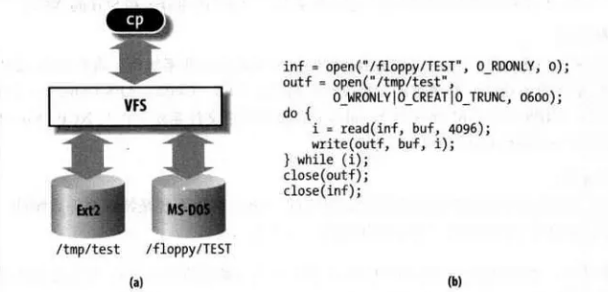
\includegraphics[width=0.5\textwidth]{figures/07-08-VFS-in-file-copy.png}
	\caption{VFS在文件复制}
	
\end{figure}

VFS的思想是把不同类型文件的共同信息放入内核,具体思路是通过在用户进程和文件系统之间引入了一个抽象层。
用户可以通过这个抽象层的接口自由使用不同的文件系统,而新的文件系统只需要支持这些接口就能直接加载到内核中使用。

\begin{figure}[ht]
	\centering
	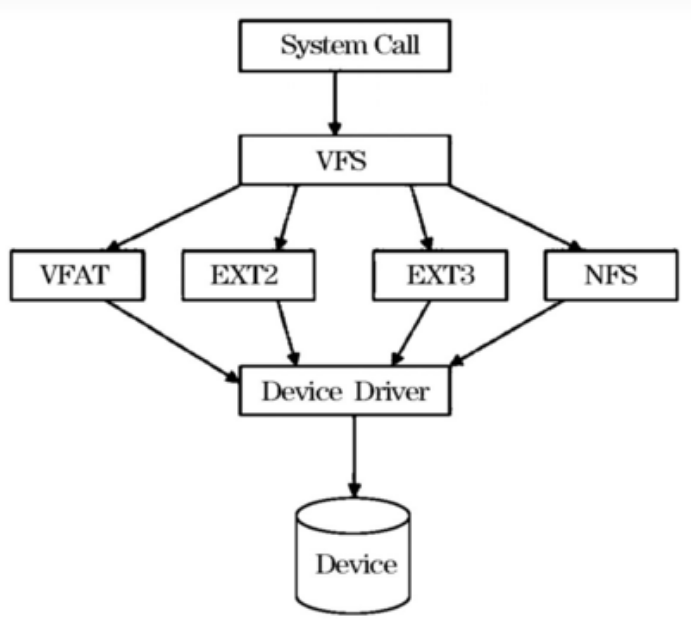
\includegraphics[width=0.5\textwidth]{figures/07-08-VFS-in-OS.png}
	\caption{VFS在OS结构中}
	
\end{figure}

\subsection{虚拟文件系统的组成}

为了实现对于不同文件系统的抽象,虚拟文件系统则需要通过数据结构完成对于不同文件系统的统一描述。在linux中为了实现这一点,定义了以下内容:

\begin{itemize}
	\item {超级块(super block)}
	超级块用于存储已安装的文件系统的相关信息。因此一个超级块可代表一个文件系统。文件系统的任意元数据修改都要修改超级块。超级块对象是常驻内
	存并被缓存的。该列表以链式方式维护在内存中,为所有进程可见。
	\item {目录项}
	目录项模块,管理路径的目录项,存储这个目录下的所有的文件的inode号和文件名等信息。其内部是
	树形结构,操作系统检索一个文件,都是从根目录开始,按层次解析路径中的所有目录,直到定位到
	文件。
	\item {inode}
	存放具体文件的一般信息(内核在操作文件或目录时需要的全部信息)。一个索引节点代表文件系统中的一个文件,但是索引节点仅当文件被访问时,才在内存中创建
	\item {文件对象}
	它代表由进程打开的文件。存放打开文件与进程之间进行交互的有关信息。这些信息仅当进程访问文件期间存放在内核中。
	这类信息仅当进程访问期间存在于内核内存中。文件对象(不是物理文件)由相应的open()系统调用创建,由close()系统调用撤销。
\end{itemize}

在NPUcore中,各部分由相应的数据结构实现。

对于超级块,NPUcore中在虚拟文件系统中定义了一个filesystem结构体,用来存储文件系统的信息。这个结构体较为简单。由于NPUcore暂时只支持FAT32文件系统,所以文件系统的类型的枚举类型只有两个值。
具体代码如下:

\begin{lstlisting}[language={Rust},caption={filesystem}]
	pub enum FS {
		Null,
		Fat32,
	}
	
	pub struct FileSystem {
		pub fs_id: usize,
		pub fs_type: FS,
	}
\end{lstlisting}

对于目录项和inode,NPUcore使用了DirectoryTreeNode结构体。不难发现,这里既有相关目录的下文件的部分,又有相关文件的信息。定义如下:

\begin{lstlisting}[language={Rust}, caption={DirectoryTreeNode}]
	pub struct DirectoryTreeNode {
		/// If this is a directory
		/// 1. cwd
		/// 2. mount point
		/// 3. root node
		/// If this is a file
		/// 1. executed by some processes
		/// This parameter will add 1 when opening
		spe_usage: Mutex<usize>,
		name: String,
		filesystem: Arc<FileSystem>,
		file: Arc<dyn File>,
		selfptr: Mutex<Weak<Self>>,
		father: Mutex<Weak<Self>>,
		children: RwLock<Option<BTreeMap<String, Arc<Self>>>>,
	}
\end{lstlisting}

从结构可以看出,这里实现了一个树形结构,指向子节点并带有路径,同时还有指向文件和文件系统的Arc指针。

对于文件对象,使用了文件描述符file\_description。定义如下:

\begin{lstlisting}[language={Rust},caption={DirectoryTreeNode}]
	#[derive(Clone)]
	pub struct FileDescriptor {
		cloexec: bool,
		nonblock: bool,
		pub file: Arc<dyn File>,
	}
\end{lstlisting}

从表面上看这些和多文件系统共存没有关系,但是以下代码完成了该项功能:
\begin{lstlisting}[language={Rust}, caption={file\_trait}]
	pub trait File: DowncastSync {
		fn deep_clone(&self) -> Arc<dyn File>;
		fn readable(&self) -> bool;
		fn writable(&self) -> bool;
		fn read(&self, offset: Option<&mut usize>, buf: &mut [u8]) -> usize;
		fn write(&self, offset: Option<&mut usize>, buf: &[u8]) -> usize;
		fn r_ready(&self) -> bool;
		fn w_ready(&self) -> bool;
		fn read_user(&self, offset: Option<usize>, buf: UserBuffer) -> usize;
		fn write_user(&self, offset: Option<usize>, buf: UserBuffer) -> usize;
		fn get_size(&self) -> usize;
		fn get_stat(&self) -> Stat;
		fn get_file_type(&self) -> DiskInodeType;
		fn is_dir(&self) -> bool {
			self.get_file_type() == DiskInodeType::Directory
		}
		fn is_file(&self) -> bool {
			self.get_file_type() == DiskInodeType::File
		}
		fn info_dirtree_node(&self, dirnode_ptr: Weak<DirectoryTreeNode>);
		fn get_dirtree_node(&self) -> Option<Arc<DirectoryTreeNode>>;
		/// open
		fn open(&self, flags: OpenFlags, special_use: bool) -> Arc<dyn File>;
		fn open_subfile(&self) -> Result<Vec<(String, Arc<dyn File>)>, isize>;
		/// create
		fn create(&self, name: &str, file_type: DiskInodeType) -> Result<Arc<dyn File>, isize>;
		fn link_child(&self, name: &str, child: &Self) -> Result<(), isize>
		where
		Self: Sized;
		/// delete(unlink)
		fn unlink(&self, delete: bool) -> Result<(), isize>;
		/// dirent
		fn get_dirent(&self, count: usize) -> Vec<Dirent>;
		/// offset
		fn get_offset(&self) -> usize {
			self.lseek(0, SeekWhence::SEEK_CUR).unwrap()
		}
		fn lseek(&self, offset: isize, whence: SeekWhence) -> Result<usize, isize>;
		/// size
		fn modify_size(&self, diff: isize) -> Result<(), isize>;
		fn truncate_size(&self, new_size: usize) -> Result<(), isize>;
		// time
		fn set_timestamp(&self, ctime: Option<usize>, atime: Option<usize>, mtime: Option<usize>);
		/// cache
		fn get_single_cache(&self, offset: usize) -> Result<Arc<Mutex<PageCache>>, ()>;
		fn get_all_caches(&self) -> Result<Vec<Arc<Mutex<PageCache>>>, ()>;
		/// memory related
		fn oom(&self) -> usize;
		/// poll, select related
		fn hang_up(&self) -> bool;
		/// iotcl
		fn ioctl(&self, _cmd: u32, _argp: usize) -> isize {
			ENOTTY
		}
		/// fcntl
		fn fcntl(&self, cmd: u32, arg: u32) -> isize;
	}
\end{lstlisting}

这在rust语法中属于特性,可以实现泛型。无论文件系统的文件结构如何定义,只要实现了这些特性,虚拟文件系统就可以识别并进行操作,很好地完成了这一点。这里不得不感叹rust语法的巧妙所在。

\subsection{虚拟文件系统提供的接口}

\begin{itemize}
	\item \texttt{sys\_openat}: 
	\begin{lstlisting}[language=rust]
		pub fn sys_openat(dirfd: usize, path: *const u8, flags: u32, mode: u32)
	\end{lstlisting}
	该接口接收来自用户空间的参数,包括目录描述符 dirfd、路径 path、打开标志位 flags 和文件权限 mode。它会根据传入的目录描述符选择要打开的文件描述符,并通过文件描述符的 open() 方法尝试打开文件。如果打开失败,则返回相应的错误码。然后,函数将新打开的文件描述符插入到当前任务的文件描述符表中,并返回新文件描述符的整数值
	\item \texttt{sys\_close}: 
	\begin{lstlisting}[language=rust]
		pub fn sys_close(fd: usize)
	\end{lstlisting}
	该接口会将进程控制块中的文件描述符表对应的一项改为 None ,代表它已经空闲,同时这也会导致内层的引用计数类型 Arc 被销毁,会减少一个文件的引用计数,当引用计数减少到 0 之后文件所占用的资源就会被自动回收。
	\item \texttt{sys\_read}: 
	\begin{lstlisting}[language=rust]
		pub fn sys_read(fd: usize, buf: usize, count: usize)
	\end{lstlisting}
	该接口根据文件描述符 fd 在文件描述符表中找到相应的文件描述符对象,使用文件描述符的 read\_user() 方法尝试从文件中读取数据到用户空间的缓冲区 buf 中,读取count个字节。
	\item \texttt{sys\_write}: 
	\begin{lstlisting}[language=rust]
		pub fn sys_write(fd: usize, buf: usize, count: usize)
	\end{lstlisting}
	该接口根据文件描述符 fd 在文件描述符表中找到相应的文件描述符对象,使用文件描述符的 write\_user() 方法尝试从文件中写入数据到用户空间的缓冲区 buf 中,共写count个字节。
	\item \texttt{sys\_fstat}: 
	\begin{lstlisting}[language=rust]
		pub fn sys_fstat(fd: usize, statbuf: *mut u8)
	\end{lstlisting}
	该接口根据文件描述符 fd 在文件描述符表中找到相应的文件描述符对象,并根据文件描述符提供的方法将文件信息写入缓冲区 statbuf 中。
	\item \texttt{sys\_mount}: 
	\begin{lstlisting}[language=rust]
		pub fn sys_mount(source: *const u8,target: *const u8,filesystemtype: *const u8,mountflags: usize,data: *const u8,)
	\end{lstlisting}
	该接口实现了挂载,参数中 source 为要挂载的文件系统的源路径或标识,target 为文件系统将要挂载到的目标位置,filesystemtype 为要挂载的文件系统的类型,mountflags是挂载选项和标志,data 为挂载所需的其他数据。
	\item \texttt{sys\_lseek}: 
	\begin{lstlisting}[language=rust]
		pub fn sys_lseek(fd: usize, offset: isize, whence: u32)
	\end{lstlisting}
	该接口根据文件描述符 fd 在文件描述符表中找到相应的文件描述符对象,然后以 whence 为偏移的基准,offset 为偏移量,返回操作后的文件指针位置。
	\item \texttt{sys\_mkdirat}: 
	\begin{lstlisting}[language=rust]
		pub fn sys_mkdirat(dirfd: usize, path: *const u8, mode: u32)
	\end{lstlisting}
	该接口在指定路径 dirfd 下创建路径为 path 的目录。
\end{itemize}